%% All tables in tables/ and figures in figs/ (except figs/MG.png) are generated by the
%% replication package (python main.py; see README.md).
\documentclass[final,3p,times,authoryear]{elsarticle}

\usepackage{amssymb}
\usepackage{amsmath}
\usepackage{booktabs}
\usepackage{caption}
\usepackage{multirow}
\usepackage[flushleft]{threeparttable}
\usepackage{float}
\usepackage{graphicx}
\usepackage{subcaption}
\usepackage{iftex}
\ifXeTeX   % Times text when compiled with XeLaTeX/tectonic (pdfLaTeX uses the class's times option)
    \usepackage{fontspec}
    \setmainfont{texgyretermes}[Extension=.otf, UprightFont=*-regular, BoldFont=*-bold,
                                ItalicFont=*-italic, BoldItalicFont=*-bolditalic]
\fi

\begin{document}

\begin{frontmatter}

\title{Size, sunshine or income? Targeting residential solar subsidies in Brazil}

\author[inst1]{Igor Westphal}
\affiliation[inst1]{organization={Department of Economics, Rice University},
            city={Houston},
            state={Texas}}

\begin{abstract}
Many developing countries have abundant sunshine but few residential solar panels. If a regulator subsidizes adoption to maximize solar generation, should it target sunny places, particular demographic groups or particular installation sizes? I estimate a discrete choice model of rooftop solar adoption for four installation sizes in the Brazilian state of Minas Gerais and embed it in the problem of a regulator who chooses upfront subsidies to maximize generation subject to a budget. Size-specific subsidies lower the public cost of each additional MWh of yearly generation by 18--33\% relative to a uniform subsidy; targeting irradiation adds about 1\% or less. Demographics matter only through price sensitivity: households in the poorest quarter of sectors are 2.5 times as price sensitive as those in the richest, and exploiting this lowers the cost per MWh by a further 6--20\%. A simple rule derived from the regulator's optimality conditions, which pays a subsidy proportional to the expected generation of an installation minus a deductible equal to the cost of inducing one adoption, captures all of these gains.
\end{abstract}

\begin{keyword}
Residential Solar Panels \sep Discrete Choice Model \sep Green Subsidies \sep Targeting
\JEL Q42 \sep Q58 \sep H23
\end{keyword}

\end{frontmatter}

\section{Introduction}
\label{Introduction}

    Many developing countries have abundant sunshine but few residential solar panels, because installation costs are high relative to incomes. Governments that want to accelerate adoption with subsidies face a design question: should they target the places where panels generate more electricity, the households that are most responsive to subsidies, or the installations that generate more per adopter? Targeting along any of these dimensions is feasible, since irradiation maps, census data and installation sizes are all observable, but it is not obvious which dimensions pay off.

    This paper answers that question for most of the Brazilian state of Minas Gerais, a region of about 30,000 census sectors where the expected output of a solar panel varies by up to 35\% across locations and where incomes vary widely. I estimate a static multinomial logit model in which households in each sector choose between not adopting and adopting one of four installation sizes (2, 4, 6 or 8 kW), as a function of prices and sector characteristics. I then embed the estimated demand in the problem of a regulator who chooses upfront subsidies to maximize the yearly generation of the panels installed, subject to a budget, and compare subsidies that vary with installation size, irradiation and demographics.

    The paper has four findings. First, conditional on prices, adoption is higher in sectors with more middle-income and literate households, and in sectors where others have already adopted. Second, size-specific subsidies substantially reduce the public cost of solar generation: relative to a uniform subsidy, the cost of each additional MWh of yearly generation falls by 18--33\%, depending on the budget. Third, targeting irradiation adds about 1\% or less to the generation gains, and targeting demographics adds nothing as long as all households are equally sensitive to prices. Fourth, they are not: price sensitivity falls steeply with income, and households in the poorest quarter of sectors are 2.5 times as price sensitive as those in the richest. Exploiting this difference lowers the cost per MWh by a further 6--20\%.

    A simple approximation to the regulator's optimality conditions explains these results and turns them into a policy rule. When adoption probabilities are small, as in the data, the cost of inducing one additional adoption is approximately the inverse of the price coefficient, $1/|\beta|$, because most of each subsidy is paid to households that would adopt anyway. The optimal subsidy is then approximately the expected generation of the installation, valued at the shadow price of the budget, minus this cost. Installation size changes expected generation four-fold, irradiation only modestly, and demographics not at all; demographics matter only through $|\beta|$. A one-parameter rule built on this approximation, which pays a subsidy proportional to expected generation minus a deductible equal to $1/|\beta|$ in the household's income group, does at least as well as all the targeted schemes, including one with 256 subsidy levels.

    Most work on the design of residential solar subsidies studies the United States \citep{hughes2015getting, dgv2019pv_discountfactor, snashallwoodhams, burr2020pv_subsidies} or other developed countries \citep{feger2020pv_welfare}. The paper also relates to work on tagging and targeting subsidies \citep{allcott2015tagging, snashallwoodhams}, geographically differentiated policies \citep{miller2019managed_competition}, investment versus generation subsidies \citep{burr2020pv_subsidies, dgv2019pv_discountfactor}, the demographic determinants of solar adoption \citep{kwan2012influence, assunccao2020developing, degroote2016heterogeneity} and peer effects \citep{bollinger2012peer, gillingham2017social}. My contribution is to show, for a developing country and in a transparent framework, which dimensions of targeting matter for the generation obtained per unit of public spending, why, and how to capture the gains with a simple rule.

\section{Background and Data}
\label{Data}

    Brazil's interest in residential solar is part of an effort to diversify its electricity supply away from large hydroelectric plants after a series of droughts. Net-metering rules introduced in 2012 (ANEEL Resolution 482/2012) let households inject surplus solar electricity into the grid in exchange for credits; they are the main incentive for residential solar, and there are no adoption subsidies in the study area. In 2019 Brazil ranked only 25th worldwide in installed photovoltaic capacity.\footnote{International Renewable Energy Agency, https://www.irena.org/Statistics/View-Data-by-Topic/Capacity-and-Generation/Country-Rankings}

    The study area is the service area of the largest distribution utility in the country, which covers most of Minas Gerais and serves about 20\% of Brazilian households (Figure \ref{fig:pvout_adoptions}). Tariffs are linear and equal across sectors. Adoption data from the electricity regulator (ANEEL) give the location, date and capacity of each residential installation, which I discretize into four sizes. Between 2016Q3 and 2019Q4 the area recorded 20,430 adoptions of these sizes.\footnote{A further 475 installations in a larger size category are treated as part of the outside option.} Solargis provided the expected yearly output of 1 kW of panels at each location. Adoption is not concentrated in the least sunny places: the quarter of sectors with the highest irradiation recorded 4.5 adoptions per 1,000 households, against 2.7--3.7 in the other quarters, and the share of households above one minimum wage per capita is highest in the third irradiation quartile, which contains most of the Belo Horizonte metropolitan area.

    \begin{figure}[htbp]
        \centering
        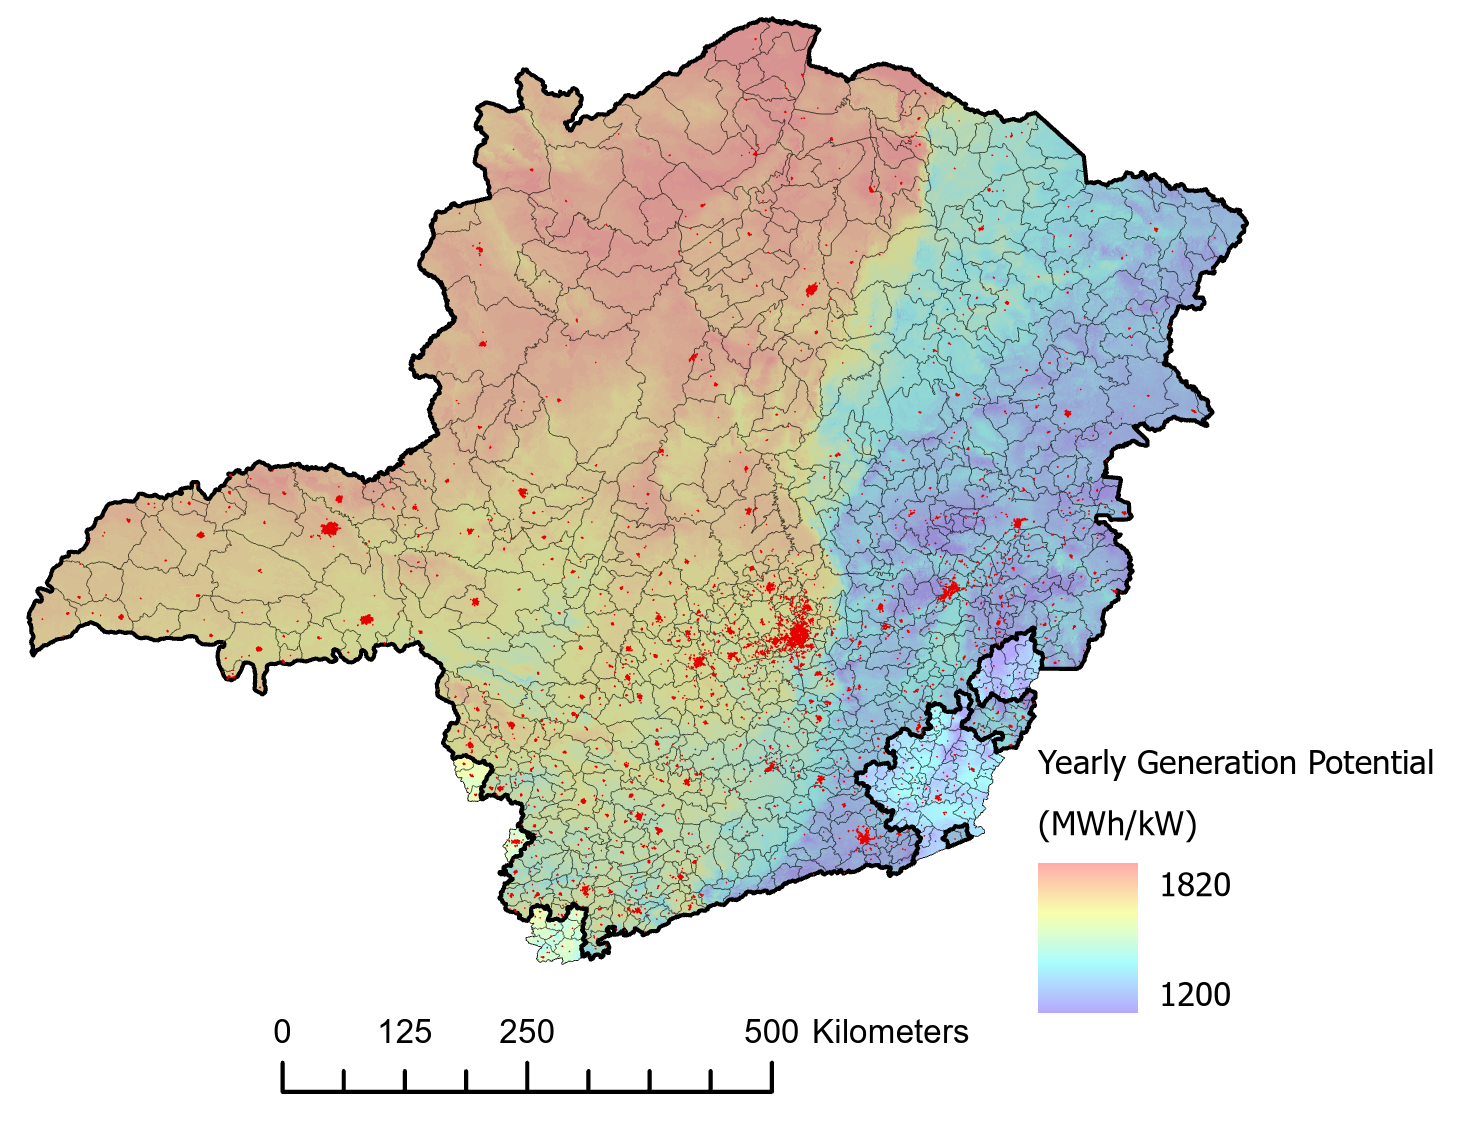
\includegraphics[width = 0.55\textwidth]{figs/MG.png}
        \caption{Study area, adoptions and generation potential. Colors show the expected yearly generation per kW installed in Minas Gerais; red dots are residential adoptions; the shaded area is the utility's service area.}
        \label{fig:pvout_adoptions}
    \end{figure}

    Demographics come from the 2010 census at the level of statistical sectors, small areas with similar numbers of households; the 29,942 sectors in the study area have 188 households on average. Installation prices come from Greener, which surveys about 850 installers twice a year, so they vary by size and over time but not across sectors. Prices fell substantially over the period, especially for larger systems, while adoptions grew rapidly (Figure \ref{fig:adoptions}). Tariffs come from ANEEL.

    \begin{figure}[htbp]
        \centering
        \begin{subfigure}[b]{0.45\textwidth}
            \centering
            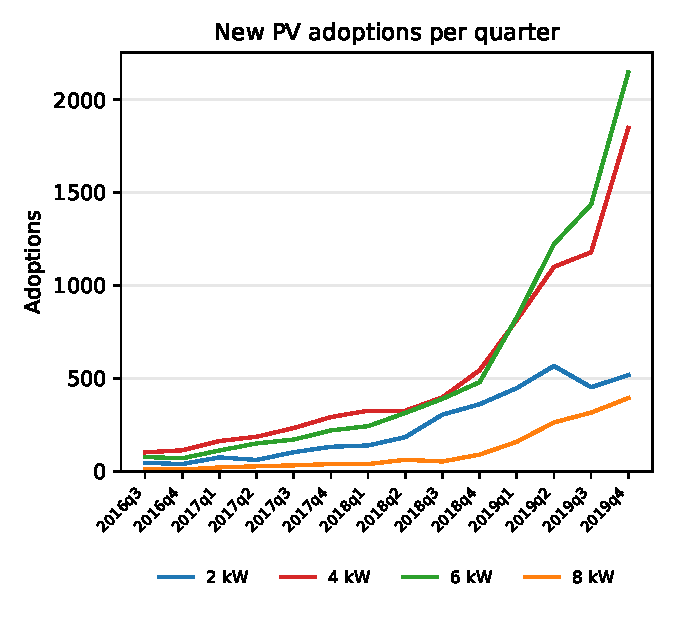
\includegraphics[width=\textwidth]{figs/newpv.pdf}
        \end{subfigure}
        \hfill
        \begin{subfigure}[b]{0.45\textwidth}
            \centering
            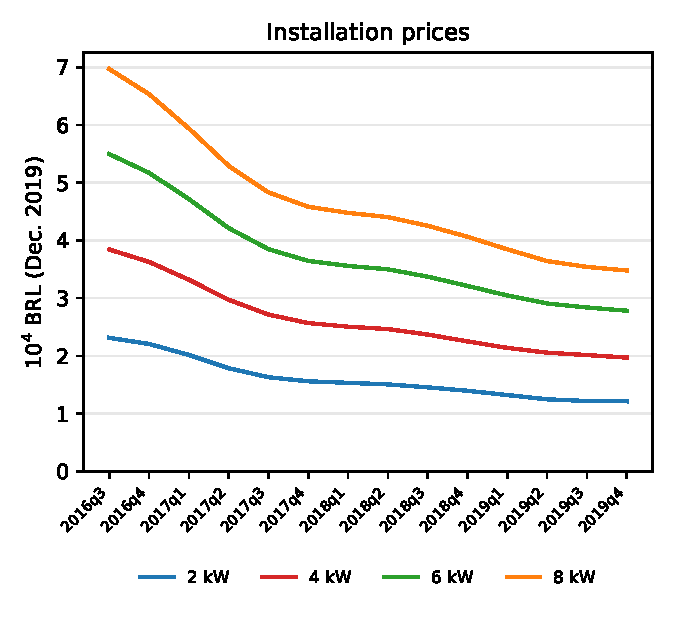
\includegraphics[width=\textwidth]{figs/prices.pdf}
        \end{subfigure}
        \caption{New residential adoptions per quarter (left) and installation prices in December 2019 BRL (right), by size.}
        \label{fig:adoptions}
    \end{figure}

    Table \ref{tab:sum} summarizes the data. I estimate the model on a random half of the sectors (15,065 sectors, 210,910 sector-quarters) and keep the other half to assess out-of-sample fit; the counterfactuals use all sectors. ``Medium income'' and ``high income'' are the shares of households with monthly per capita income between one and five, and above five, 2010 minimum wages. ``Bathrooms'' (per household) proxies dwelling size and electricity use, and ``houses'' is the share of households living in houses rather than apartments, which matters for roof space. The ``stock of PVs'' is the cumulative number of installations in the sector before the quarter.

    \begin{table}[htbp]
\centering
\small
\begin{threeparttable}
\caption{Summary Statistics}
\label{tab:sum}
\begin{tabular}{lcccccc}
\hline \hline \noalign{\vskip 1mm}
\textbf{Variable} & \textbf{Mean} & \textbf{SD} & \textbf{Min} & \textbf{Median} & \textbf{Max} & \textbf{N} \\ \hline \noalign{\vskip 1mm}
\multicolumn{7}{l}{\textit{Adoptions per sector-quarter}} \\
2 kW & 0.008 & 0.097 & 0 & 0 & 7 & 419,188 \\
4 kW & 0.018 & 0.156 & 0 & 0 & 17 & 419,188 \\
6 kW & 0.019 & 0.168 & 0 & 0 & 11 & 419,188 \\
8 kW & 0.004 & 0.064 & 0 & 0 & 6 & 419,188 \\
\multicolumn{7}{l}{\textit{Investment price ($10^4$ BRL)}} \\
2 kW & 1.600 & 0.357 & 1.212 & 1.519 & 2.312 & 14 \\
4 kW & 2.629 & 0.602 & 1.970 & 2.485 & 3.842 & 14 \\
6 kW & 3.736 & 0.865 & 2.782 & 3.529 & 5.495 & 14 \\
8 kW & 4.704 & 1.104 & 3.479 & 4.441 & 6.969 & 14 \\
\multicolumn{7}{l}{\textit{Sector characteristics}} \\
Households (2016Q3) & 188 & 93 & 5 & 187 & 845 & 29,942 \\
Density ($10^4$ hab/km$^2$) & 0.538 & 0.841 & 0.000 & 0.315 & 42 & 29,942 \\
Medium income (share) & 0.314 & 0.183 & 0 & 0.296 & 1 & 29,942 \\
High income (share) & 0.040 & 0.094 & 0 & 0.009 & 0.949 & 29,942 \\
Bathrooms & 1.312 & 0.425 & 0 & 1.225 & 5.866 & 29,942 \\
Age (decades) & 3.354 & 0.409 & 1.729 & 3.322 & 6.222 & 29,942 \\
Literacy (share) & 0.846 & 0.082 & 0.056 & 0.862 & 1 & 29,942 \\
Houses (share) & 0.912 & 0.208 & 0 & 1 & 1 & 29,942 \\
Stock of PVs before the quarter & 0.179 & 0.983 & 0 & 0 & 87 & 419,188 \\
Solar generation (MWh/kW/year) & 1.600 & 0.093 & 1.320 & 1.630 & 1.790 & 29,942 \\
Electricity tariff (BRL/kWh) & 0.838 & 0.053 & 0.760 & 0.851 & 0.914 & 14 \\
\noalign{\vskip 1mm} \hline
\end{tabular}
\begin{tablenotes}
\footnotesize
\item All 29,942 sectors over 14 quarters (2016Q3--2019Q4). Households are those that had not adopted at the start of the period. Prices and tariffs are common to the whole area. December 2019 BRL.
\end{tablenotes}
\end{threeparttable}
\end{table}


\section{Model}
\label{Model}

\subsection{Demand}

    In each quarter $t$, each of the $L_{mt}$ households in sector $m$ that have not yet adopted chooses between not adopting ($j=0$) and adopting one of $J=4$ sizes. Adopting size $j$ yields utility
    \begin{equation}
        u_{imjt} = \beta_m\, p_{jt} + \delta_t + w_{mt}^{\prime} \gamma_{j} + \varepsilon_{imjt},
        \label{eq:utility}
    \end{equation}
    where $p_{jt}$ is the price, $\delta_t$ a quarter fixed effect common to all sizes, $w_{mt}$ a vector of sector characteristics including a constant, and $\varepsilon_{imjt}$ a type I extreme value shock; the utility of not adopting is normalized to zero. The coefficients $\gamma_j$ differ across sizes, so sector characteristics can affect both whether and how much capacity households install. The quarter fixed effects absorb anything that changes the attractiveness of solar over time for all sizes alike, such as awareness, financing conditions or the electricity tariff, so that the price coefficient is identified from changes in relative prices across sizes. In the main specification $\beta_m = \beta$; I also let it differ across quartiles of the share of households above one minimum wage. Households leave the market after adopting (fewer than 1\% appear more than once in the data). The probability of adopting size $j$ is
    \begin{equation}
        s_{mjt} = \frac{\exp \left(\beta_m p_{jt} + \delta_t + w_{mt}^{\prime} \gamma_{j}\right)}{1+\sum_{k=1}^{J} \exp \left(\beta_m p_{kt} + \delta_t + w_{mt}^{\prime} \gamma_{k}\right)}.
        \label{eq:ccp}
    \end{equation}
    With $y_{mjt}$ adoptions of size $j$ and $y_{m0t} = L_{mt} - \sum_j y_{mjt}$, I estimate the parameters by maximizing the log-likelihood $\sum_{m,j,t} y_{mjt} \log s_{mjt}$ over the estimation sample. As shown by \citet{baker1994multinomial}, this is numerically equivalent to a Poisson regression of the counts on the same regressors with a fixed effect for each sector and quarter, which I use for computation. Because unobservables are likely persistent within sectors, I report standard errors clustered by sector.

\subsection{The regulator's problem}

    Following \citet{feger2020pv_welfare}, a regulator chooses upfront subsidies $c_{mj} \geq 0$ per installation, which lower the price paid by households to $p_{jt} - c_{mj}$. The yearly generation of the panels installed in quarter $t$ is
    \begin{equation}
        P_{t}(c) = \sum_{m=1}^{M} I_{m}\, L_{mt} \sum_{j=1}^{J} \kappa_{j}\, s_{mjt}(c),
        \label{eq:elprod}
    \end{equation}
    where $I_m$ is the expected yearly output per kW in sector $m$ and $\kappa_j$ the capacity of size $j$.\footnote{The net present value of this generation over a lifetime of $R$ years with discount factor $\delta$ is $\rho \sum_t P_t(c)$ with $\rho = (1-\delta^{R})/(1-\delta)$, a constant that does not affect the solution.} The regulator solves
    \begin{equation}
        \max _{c \geq 0} \; \sum_{t} P_{t}(c) \quad \text{s.t.} \quad \sum_{t,m,j} c_{mj}\, L_{mt}\, s_{mjt}(c) \leq B,
        \label{eq:regulator}
    \end{equation}
    paying the subsidy to every adopter, including those who would have adopted anyway. I consider subsidies that are equal within groups of sectors (quartiles of irradiation or of demographic characteristics) and simple rules that set the subsidy of each sector as a function of its irradiation. The grouped problems are not concave in general; I solve them by sequential quadratic programming with analytic gradients.

\subsection{What drives optimal targeting}
\label{sec:mechanism}

    Let $c_{jg}$ be the subsidy for size $j$ in a group $g$ of sectors with common price coefficient $\beta_g$. Since $\partial s_{mkt}/\partial c_{jg} = |\beta_g|\, s_{mkt}(\mathbf{1}\{k=j\} - s_{mjt})$ for $m \in g$, and adoption probabilities are tiny (about 0.02\% per quarter on average), the generation bought by the marginal BRL spent on $c_{jg}$ is approximately $|\beta_g|\, \kappa_j \bar I_{jg} / (1 + |\beta_g| c_{jg})$, where $\bar I_{jg}$ is the adoption-weighted irradiation of group $g$. Setting it equal to the shadow value of the budget, $\lambda$, gives
    \begin{equation}
        c^{*}_{jg} \approx \max\left\{0,\; \frac{\kappa_j\, \bar I_{jg}}{\lambda} - \frac{1}{|\beta_g|}\right\}.
        \label{eq:approx}
    \end{equation}
    The optimal subsidy is the expected yearly generation of an installation, $\kappa_j \bar I_{jg}$, valued at $1/\lambda$, minus $1/|\beta_g|$. This second term is the cost of inducing one more adoption with a small subsidy: a subsidy of one BRL raises the adoption probability by the fraction $|\beta_g|$ (per $10^4$ BRL) but is paid to every adopter, so each induced adoption costs about $1/|\beta_g|$. Equation (\ref{eq:approx}) has three implications. Targeting a characteristic pays off only if it changes expected generation per installation or the price sensitivity of households. Sector characteristics that shift the level of adoption but not price sensitivity, however strongly they predict adoption, do not matter. And the optimum can be approximated by a one-parameter rule, $c_{mj} = \max\{0, a\, \kappa_j I_m - 1/|\beta_m|\}$, with $a$ set to exhaust the budget.

\section{Results}
\label{Results}

    Table \ref{tab:results} reports the estimates of the main specification. The price coefficient is $-0.53$ and significant. Without quarter fixed effects it is twice as large (Table \ref{tab:specs}, column 1), which indicates that part of the growth of adoption over the period, which coincided with falling prices, reflects common trends rather than responses to prices. The main specification identifies the price coefficient only from relative price changes and is therefore more conservative. Standard errors clustered by sector are larger than conventional ones, but most coefficients remain significant.

    \begin{table}[htbp]
\centering
\small
\begin{threeparttable}
\caption{Estimation Results}
\label{tab:results}
\begin{tabular}{lllll}
\hline \hline \noalign{\vskip 1mm}
Investment price ($10^4$ BRL) & -0.529*** & & & \\
 & (0.099) & & & \\
 & [0.083] & & & \\
 & \textbf{2 kW} & \textbf{4 kW} & \textbf{6 kW} & \textbf{8 kW} \\ \cline{2-5} \noalign{\vskip 1mm}
Constant & -15.141*** & -11.623*** & -10.079*** & -10.796*** \\
 & (0.740) & (0.587) & (0.697) & (1.029) \\
 & [0.683] & [0.527] & [0.570] & [0.964] \\
Log(1 + stock of PVs) & 0.812*** & 0.860*** & 1.112*** & 1.027*** \\
 & (0.073) & (0.073) & (0.090) & (0.095) \\
 & [0.040] & [0.025] & [0.024] & [0.054] \\
Density ($10^4$ hab/km$^2$) & -0.912*** & -0.913*** & -0.868*** & -1.032*** \\
 & (0.081) & (0.058) & (0.068) & (0.136) \\
 & [0.074] & [0.051] & [0.053] & [0.122] \\
Medium income (share) & 2.099*** & 3.011*** & 1.603*** & 0.992** \\
 & (0.285) & (0.234) & (0.336) & (0.422) \\
 & [0.257] & [0.172] & [0.171] & [0.377] \\
High income (share) & 0.968 & 0.996 & -1.325 & -1.581 \\
 & (0.868) & (0.722) & (0.854) & (1.199) \\
 & [0.635] & [0.400] & [0.367] & [0.811] \\
Bathrooms & 0.026 & 0.257* & 0.759*** & 0.846*** \\
 & (0.187) & (0.140) & (0.183) & (0.259) \\
 & [0.136] & [0.085] & [0.077] & [0.169] \\
Age (decades) & -0.410*** & -0.237*** & 0.176* & 0.218* \\
 & (0.102) & (0.086) & (0.101) & (0.131) \\
 & [0.077] & [0.051] & [0.049] & [0.110] \\
Literacy (share) & 5.377*** & 1.313** & -0.497 & -0.610 \\
 & (0.905) & (0.609) & (0.707) & (1.067) \\
 & [0.803] & [0.521] & [0.497] & [1.055] \\
Houses (share) & 1.434*** & 1.386*** & 0.162 & -0.133 \\
 & (0.248) & (0.172) & (0.195) & (0.369) \\
 & [0.210] & [0.137] & [0.124] & [0.277] \\
\hline \noalign{\vskip 1mm}
Quarter fixed effects & \multicolumn{4}{l}{Yes} \\
Log-likelihood & \multicolumn{4}{l}{-94,617.4} \\
Sector-quarters & \multicolumn{4}{l}{210,910} \\
\noalign{\vskip 1mm} \hline
\end{tabular}
\begin{tablenotes}
\footnotesize
\item Maximum likelihood estimates on the estimation sample (15,065 sectors, 14 quarters), with quarter fixed effects common to all sizes (which absorb the electricity tariff). Standard errors clustered by sector in parentheses, conventional ones in brackets; stars refer to the clustered ones (*** $p<0.01$, ** $p<0.05$, * $p<0.1$). No adoption is the reference alternative.
\end{tablenotes}
\end{threeparttable}
\end{table}


    Adoption increases with the number of earlier installations in the sector: a first installation raises the probability of adoption by 76--116\%, depending on the size. This is consistent with peer effects, although the stock also captures persistent unobserved sector characteristics, so I do not interpret it causally. Density reduces the adoption of all sizes, consistent with the need for roof space, and bathrooms increase adoption, more so for larger sizes, consistent with larger dwellings consuming more electricity. The share of middle-income households increases the adoption of all sizes. Literacy strongly increases the adoption of 2 and 4 kW systems, consistent with information facilitating the take-up of new technologies, and the share of houses increases the adoption of the smaller sizes. Older residents adopt fewer small and more large systems.

    \begin{table}[htbp]
\centering
\small
\begin{threeparttable}
\caption{Price Coefficients Across Specifications}
\label{tab:specs}
\begin{tabular}{lccc}
\hline \hline \noalign{\vskip 1mm}
 & (1) & (2) & (3) \\ \hline \noalign{\vskip 1mm}
Price & -1.120*** & -0.529*** & -0.438*** \\
 & (0.053) & (0.099) & (0.099) \\
Price $\times$ income Q1 &  &  & -0.661*** \\
 &  &  & (0.059) \\
Price $\times$ income Q2 &  &  & -0.285*** \\
 &  &  & (0.038) \\
Price $\times$ income Q3 &  &  & -0.093*** \\
 &  &  & (0.026) \\
\noalign{\vskip 1mm}
Quarter fixed effects & No & Yes & Yes \\
Log-likelihood & -94,722.8 & -94,617.4 & -94,359.3 \\
Hold-out adoptions, predicted & 10,448 & 10,424 & 10,403 \\
Hold-out adoptions, observed & \multicolumn{3}{c}{10,331} \\
\noalign{\vskip 1mm} \hline
\end{tabular}
\begin{tablenotes}
\footnotesize
\item All specifications include the sector characteristics of Table \ref{tab:results} with size-specific coefficients; (1) also includes the electricity tariff. In (3) the price coefficient differs across quartiles of the share of households with per capita income above one minimum wage; ``Price'' is the coefficient of the richest quartile and the interactions are differences relative to it. Clustered standard errors in parentheses. The hold-out sample consists of the 14,877 sectors not used in estimation.
\end{tablenotes}
\end{threeparttable}
\end{table}


    Table \ref{tab:specs} compares specifications. All three predict adoptions in the hold-out sample of sectors to within about 1\%. Column 3 lets the price coefficient differ across income quartiles. Price sensitivity falls steeply with income: the coefficient is $-1.10$ in the poorest quartile, $-0.72$ and $-0.53$ in the middle ones and $-0.44$ in the richest, so the poorest households are 2.5 times as price sensitive as the richest. Figure \ref{fig:datafit} shows that the main specification also tracks the evolution of adoptions over time, in and out of sample.

    \begin{figure}[htbp]
        \centering
        \begin{subfigure}[b]{0.48\textwidth}
            \centering
            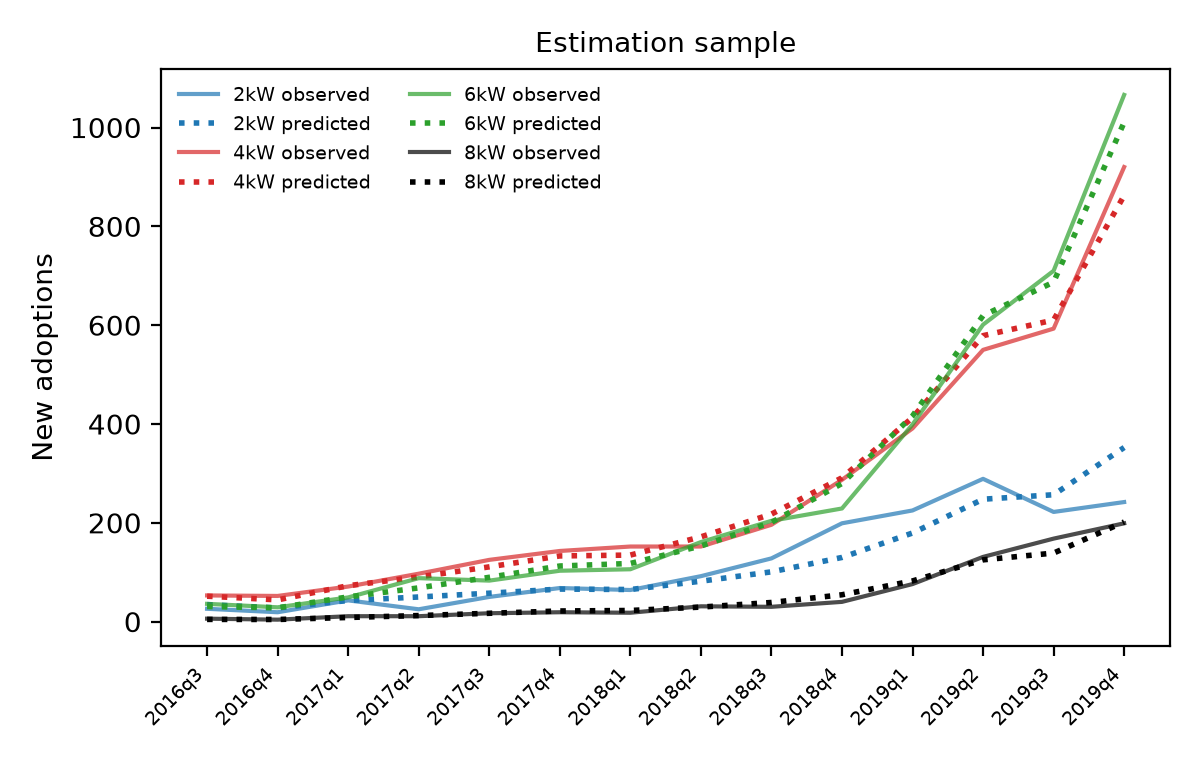
\includegraphics[width=\textwidth]{figs/datafit_in.png}
        \end{subfigure}
        \hfill
        \begin{subfigure}[b]{0.48\textwidth}
            \centering
            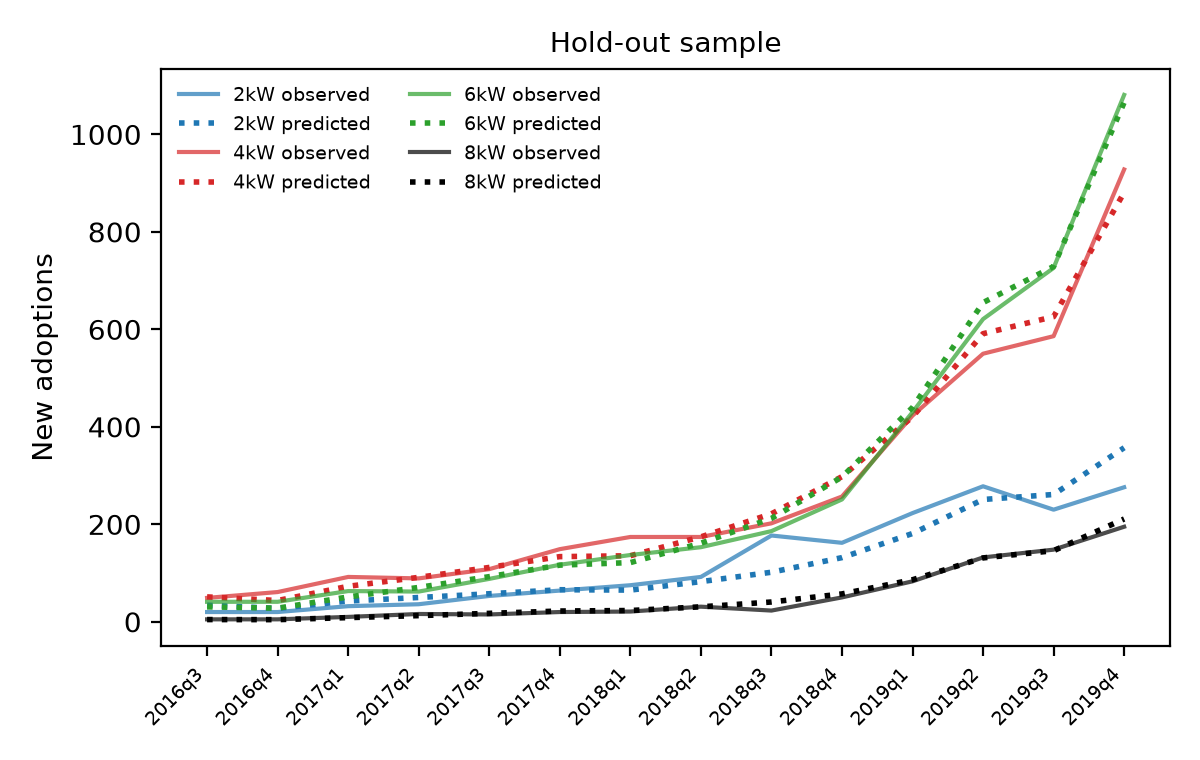
\includegraphics[width=\textwidth]{figs/datafit_out.png}
        \end{subfigure}
        \caption{Predicted (dotted) and observed (solid) adoptions per quarter, in the estimation sample (left) and in the hold-out sample of sectors not used in estimation (right), main specification.}
        \label{fig:datafit}
    \end{figure}

    \begin{table}[htbp]
\centering
\small
\begin{threeparttable}
\caption{Mean Price Elasticities}
\label{tab:mean_price_elasticity}
\begin{tabular}{lcccc}
\hline \hline \noalign{\vskip 1mm}
 & \textbf{2 kW} & \textbf{4 kW} & \textbf{6 kW} & \textbf{8 kW} \\ \hline \noalign{\vskip 1mm}
\textbf{2 kW} & -0.8459 & 0.0001 & 0.0001 & 0.0000 \\
\textbf{4 kW} & 0.0000 & -1.3903 & 0.0001 & 0.0000 \\
\textbf{6 kW} & 0.0000 & 0.0001 & -1.9755 & 0.0000 \\
\textbf{8 kW} & 0.0000 & 0.0001 & 0.0001 & -2.4875 \\
\noalign{\vskip 1mm} \hline
\end{tabular}
\begin{tablenotes}
\footnotesize
\item Elasticity of the probability of adopting the row size with respect to the price of the column size, averaged across sector-quarters of the estimation sample (specification of Table \ref{tab:results}).
\end{tablenotes}
\end{threeparttable}
\end{table}


    Own-price elasticities range from $-0.85$ for 2 kW systems to $-2.49$ for 8 kW systems (Table \ref{tab:mean_price_elasticity}). The difference does not mean that buyers of large systems are more price sensitive: with a common price coefficient, the own-price elasticity is $\hat\beta\, p_{jt}(1-s_{mjt}) \approx \hat\beta\, p_{jt}$, proportional to the price. The semi-elasticity is the same for all sizes: a price cut of 1,000 BRL raises the probability of adopting any size by about 5\%. Cross-price elasticities are close to zero because adoption shares are small.

    Table \ref{tab:marginal_effects_demographic_characteristics} reports the mean marginal effects of sector characteristics,
    \begin{equation}
        \label{eq:marginal_effect_demographics}
        \frac{\partial s_{mjt}}{\partial w_{mt}} = s_{mjt} \Big(\hat{\gamma}_{j} - \sum_{\ell=1}^{J} s_{m\ell t}\, \hat{\gamma}_{\ell}\Big).
    \end{equation}
    They are small in absolute terms because adoption probabilities are small (0.004, 0.009, 0.009 and 0.002 percentage points per quarter for the four sizes), but large in relative terms. Recomputing the probabilities for discrete changes in all sectors, a ten-percentage-point increase in the share of middle-income households raises the mean probability of adopting a 2, 4, 6 or 8 kW system by 23\%, 35\%, 17\% and 10\%; the same increase in literacy raises it by 71\% for 2 kW and 14\% for 4 kW systems; one standard deviation more density reduces it by 52--58\%. Low incomes and low educational attainment are thus obstacles to adoption, both because they reduce adoption at given prices and, as Table \ref{tab:specs} shows, because they make households more sensitive to prices.

    \begin{table}[htbp]
\centering
\small
\begin{threeparttable}
\caption{Marginal Effects of Sector Characteristics}
\label{tab:marginal_effects_demographic_characteristics}
\begin{tabular}{lcccc}
\hline \hline \noalign{\vskip 1mm}
 & \textbf{2 kW} & \textbf{4 kW} & \textbf{6 kW} & \textbf{8 kW} \\ \hline \noalign{\vskip 1mm}
Log(1 + stock of PVs) & 0.0032 & 0.0076 & 0.0101 & 0.0019 \\
Density ($10^4$ hab/km$^2$) & -0.0036 & -0.0081 & -0.0079 & -0.0019 \\
Medium income (share) & 0.0084 & 0.0268 & 0.0145 & 0.0018 \\
High income (share) & 0.0039 & 0.0089 & -0.0121 & -0.0029 \\
Bathrooms & 0.0001 & 0.0023 & 0.0069 & 0.0016 \\
Age (decades) & -0.0016 & -0.0021 & 0.0016 & 0.0004 \\
Literacy (share) & 0.0215 & 0.0117 & -0.0046 & -0.0011 \\
Houses (share) & 0.0057 & 0.0123 & 0.0015 & -0.0003 \\
\noalign{\vskip 1mm} \hline
\end{tabular}
\begin{tablenotes}
\footnotesize
\item Mean across sector-quarters of Equation (\ref{eq:marginal_effect_demographics}): change in the quarterly probability of adopting each size, in percentage points, for a one-unit increase in each variable (for shares, from 0 to 1).
\end{tablenotes}
\end{threeparttable}
\end{table}


\section{Counterfactuals}
\label{Counterfactuals}

    I solve Program (\ref{eq:regulator}) for budgets between 10 and 200 million BRL under six designs: a uniform subsidy; subsidies by size; by size and irradiation quartile; by size and quartiles of density, middle-income share and bathrooms (256 subsidies); a subsidy proportional to the expected generation of each installation, $a\, \kappa_j I_m$; and the rule $\max\{0, a\, \kappa_j I_m - 1/|\beta_m|\}$ suggested by Equation (\ref{eq:approx}). Without subsidies the main specification predicts 20,523 adoptions, close to the 20,430 observed, and 157,126 MWh of yearly generation. Table \ref{tab:comparison} compares the designs under a common price coefficient (Panel A) and under price coefficients that differ by income quartile (Panel B).

    \begin{table}[htbp]
\centering
\small
\begin{threeparttable}
\caption{Generation Under Alternative Subsidy Designs}
\label{tab:comparison}
\begin{tabular}{ccccccc}
\hline \hline \noalign{\vskip 1mm}
\multicolumn{7}{l}{\textit{Panel A: common price sensitivity (Table \ref{tab:results})}} \\
\textbf{Budget} & \textbf{Uniform} & \textbf{Size} & \textbf{Size \& irr.} & \textbf{Size \& dem.} & \textbf{Prop.} & \textbf{Rule} \\ \hline \noalign{\vskip 1mm}
\multicolumn{7}{l}{Increase in yearly generation relative to no subsidy (\%)} \\
10 & 2.5 & 3.8 & 3.8 & 3.8 & 2.9 & 3.8 \\
20 & 5.0 & 7.0 & 7.1 & 7.0 & 5.6 & 7.1 \\
50 & 12.1 & 16.0 & 16.1 & 16.0 & 13.7 & 16.1 \\
100 & 23.1 & 29.3 & 29.5 & 29.3 & 26.1 & 29.5 \\
200 & 43.0 & 52.5 & 52.8 & 52.5 & 48.6 & 52.8 \\
\multicolumn{7}{l}{Public cost per additional MWh/year (BRL)} \\
10 & 2,516 & 1,676 & 1,664 & 1,675 & 2,227 & 1,663 \\
20 & 2,546 & 1,808 & 1,790 & 1,807 & 2,254 & 1,788 \\
50 & 2,630 & 1,990 & 1,975 & 1,989 & 2,330 & 1,974 \\
100 & 2,753 & 2,172 & 2,160 & 2,171 & 2,440 & 2,159 \\
200 & 2,959 & 2,424 & 2,413 & 2,423 & 2,621 & 2,412 \\
\noalign{\vskip 2mm}
\multicolumn{7}{l}{\textit{Panel B: price sensitivity by income quartile (Table \ref{tab:specs}, column 3)}} \\
\textbf{Budget} & \textbf{Uniform} & \textbf{Size} & \textbf{Size \& irr.} & \textbf{Size \& dem.} & \textbf{Prop.} & \textbf{Rule} \\ \hline \noalign{\vskip 1mm}
\multicolumn{7}{l}{Increase in yearly generation relative to no subsidy (\%)} \\
10 & 2.5 & 3.9 & 3.9 & 4.7 & 2.8 & 4.8 \\
20 & 5.0 & 7.1 & 7.2 & 8.4 & 5.6 & 8.6 \\
50 & 12.1 & 16.2 & 16.2 & 18.1 & 13.6 & 18.4 \\
100 & 23.2 & 29.7 & 29.7 & 32.1 & 26.1 & 32.5 \\
200 & 43.4 & 53.6 & 53.7 & 56.7 & 49.0 & 57.2 \\
\multicolumn{7}{l}{Public cost per additional MWh/year (BRL)} \\
10 & 2,528 & 1,654 & 1,651 & 1,357 & 2,246 & 1,332 \\
20 & 2,556 & 1,785 & 1,781 & 1,511 & 2,271 & 1,487 \\
50 & 2,634 & 1,972 & 1,970 & 1,758 & 2,340 & 1,735 \\
100 & 2,749 & 2,145 & 2,143 & 1,986 & 2,439 & 1,962 \\
200 & 2,939 & 2,377 & 2,374 & 2,250 & 2,602 & 2,227 \\
\noalign{\vskip 1mm} \hline
\end{tabular}
\begin{tablenotes}
\footnotesize
\item Uniform: one subsidy for all. Size: one subsidy per size. Size \& irr.: per size and irradiation quartile (16 subsidies). Size \& dem.: per size and quartiles of density, medium-income share and bathrooms (256 subsidies). Prop.: subsidy proportional to the expected yearly generation of the installation, $a\,\kappa_j I_m$. Rule: $\max\{0, a\,\kappa_j I_m - 1/|\beta_m|\}$, Equation (\ref{eq:approx}). In the last two, $a$ is set to exhaust the budget. Budgets in millions of December 2019 BRL. Generation without subsidies: 157,126 MWh/year (Panel A) and 156,912 MWh/year (Panel B).
\end{tablenotes}
\end{threeparttable}
\end{table}


    \textit{Uniform subsidy.} A budget of 10 million BRL finances a subsidy of 475 BRL per installation and raises generation by 2.5\%. Almost all of the money goes to households that would have adopted anyway: the subsidy induces 520 additional adoptions, so each costs about 19,200 BRL, close to $1/|\hat\beta| \approx$ 18,900 BRL plus the subsidy, as Section \ref{sec:mechanism} predicts. The share of payments that go to such households falls from 97\% at 10 million BRL to 70\% at 200 million BRL.

    \textit{Subsidies by size.} The regulator subsidizes only the largest installations (Table \ref{tab:cf1}): 8 kW systems at every budget and 6 kW systems from 20 million BRL. At 100 million BRL the 8 kW subsidy is 13,500 BRL, 29\% of the average price. Adoptions of smaller systems fall slightly as some households switch to the subsidized sizes, but generation rises much more than with a uniform subsidy, and the public cost of each additional MWh/year falls by 18--33\% (Table \ref{tab:comparison}, Panel A). A subsidy of a given amount induces roughly the same number of adoptions whatever size it is attached to, but an 8 kW system generates four times as much as a 2 kW one. A subsidy strictly proportional to expected generation does much worse than size-specific subsidies, because it pays small installations whose expected generation does not cover the fixed cost $1/|\beta|$ of inducing an adoption.

    \begin{table}[htbp]
\centering
\small
\begin{threeparttable}
\caption{Optimal Subsidies by Installation Size}
\label{tab:cf1}
\begin{tabular}{cccccccccc}
\hline \hline \noalign{\vskip 1mm}
 & \multicolumn{4}{c}{\textit{Subsidy ($10^4$ BRL)}} & \multicolumn{4}{c}{\textit{Adoptions}} & \\ \cline{2-5} \cline{6-9}
\textbf{Budget} & \textbf{2 kW} & \textbf{4 kW} & \textbf{6 kW} & \textbf{8 kW} & \textbf{2 kW} & \textbf{4 kW} & \textbf{6 kW} & \textbf{8 kW} & \textbf{\begin{tabular}[c]{@{}c@{}}Generation\\ (MWh/year)\end{tabular}} \\ \hline \noalign{\vskip 1mm}
0 & 0.00 & 0.00 & 0.00 & 0.00 & 3,400 & 7,633 & 7,934 & 1,556 & 157,126 \\
10 & 0.00 & 0.00 & 0.00 & 0.49 & 3,400 & 7,633 & 7,932 & 2,021 & 163,093 \\
20 & 0.00 & 0.00 & 0.05 & 0.70 & 3,399 & 7,632 & 8,152 & 2,252 & 168,187 \\
50 & 0.00 & 0.00 & 0.27 & 0.98 & 3,399 & 7,629 & 9,122 & 2,616 & 182,248 \\
100 & 0.00 & 0.00 & 0.54 & 1.35 & 3,397 & 7,625 & 10,544 & 3,175 & 203,172 \\
200 & 0.00 & 0.00 & 0.94 & 1.88 & 3,395 & 7,619 & 12,971 & 4,188 & 239,636 \\
\noalign{\vskip 1mm} \hline
\end{tabular}
\begin{tablenotes}
\footnotesize
\item Budgets in millions and subsidies in $10^4$ BRL per installation (December 2019 BRL). Budget $=0$ is the model prediction without subsidies (observed adoptions: 3,430, 7,624, 7,861 and 1,515). Adoptions are totals over the 14 quarters in all 29,942 sectors; generation is their yearly output.
\end{tablenotes}
\end{threeparttable}
\end{table}


    \textit{Irradiation and demographics with a common price coefficient.} Subsidies increase with irradiation (Table \ref{tab:cf2}), as Equation (\ref{eq:approx}) predicts, but targeting irradiation quartiles adds only 0.5--1.0\% to the generation gains of size-specific subsidies, because expected generation per installation differs by only 16\% between the least and the most sunny quartile. Targeting density, income and dwelling size adds less than 0.1\%: these characteristics change how many households adopt, but neither how much each installation generates nor how many additional adoptions a BRL buys. The one-parameter rule does slightly better than all targeted schemes.

    \begin{table}[htbp]
\centering
\small
\begin{threeparttable}
\caption{Optimal Subsidies by Installation Size and Irradiation Quartile}
\label{tab:cf2}
\begin{tabular}{cccccc}
\hline \hline \noalign{\vskip 1mm}
\textbf{Budget} & \textbf{Size} & \textbf{Q1} & \textbf{Q2} & \textbf{Q3} & \textbf{Q4} \\ \hline \noalign{\vskip 1mm}
\multirow{1}{*}{10} & 8 kW & 0.28 & 0.46 & 0.54 & 0.60 \\
\noalign{\vskip 1mm}
\multirow{2}{*}{50} & 6 kW & 0.07 & 0.23 & 0.31 & 0.35 \\
 & 8 kW & 0.72 & 0.94 & 1.04 & 1.11 \\
\noalign{\vskip 1mm}
\multirow{3}{*}{200} & 4 kW & 0.00 & 0.00 & 0.03 & 0.06 \\
 & 6 kW & 0.67 & 0.88 & 0.98 & 1.04 \\
 & 8 kW & 1.53 & 1.81 & 1.94 & 2.03 \\
\noalign{\vskip 1mm} \hline
\end{tabular}
\begin{tablenotes}
\footnotesize
\item Subsidies in $10^4$ BRL per installation by quartile of the sector's solar generation potential (Q1 = least sunny). Sizes that receive no subsidy in any quartile are omitted. Budgets in millions of BRL.
\end{tablenotes}
\end{threeparttable}
\end{table}


    \textit{Price sensitivity that differs by income.} When the price coefficient differs across income quartiles (Panel B), demographic targeting pays off. Subsidies by size and demographics raise the generation gain by 6--22\% relative to size-only subsidies, and the one-parameter rule, whose deductible $1/|\beta_m|$ is smaller in poorer sectors, raises it by 7--24\% and lowers the public cost per MWh by 24--47\% relative to a uniform subsidy. Poorer households adopt less, but those at the margin are cheaper to persuade, so a larger share of each subsidy goes to induced adoptions. Irradiation targeting still adds little. Appendix Table \ref{tab:comparison_nofe} shows that the results of Panel A are similar without quarter fixed effects, although all subsidies are then about twice as effective because the price coefficient is larger.

\section{Conclusion}
\label{Conclusion}

    In Minas Gerais, size-specific subsidies substantially increase the solar generation obtained from a given budget, irradiation targeting adds little, and demographic targeting pays off only because, and to the extent that, poorer households are more sensitive to prices. A simple approximation to the regulator's optimality conditions explains these results: the optimal subsidy is approximately the value of the expected generation of an installation minus the cost of inducing one adoption, which equals the inverse of the price coefficient. It also yields a simple, implementable rule: an upfront subsidy proportional to expected yearly generation, which depends only on capacity and the local irradiation map, minus a deductible that is smaller for lower-income areas. In this setting the rule captures all of the gains of much more complex targeted schemes.

    The analysis has limitations. Prices vary only over time and across sizes, so the price coefficient is identified from relative price changes across sizes; the quarter fixed effects remove common trends, but the coefficient halves when they are included, which shows that identification matters for the magnitude of all subsidy effects. The model is static, while falling prices may lead households to delay adoption \citep{dgv2019pv_discountfactor, burr2020pv_subsidies}. The logit model implies that substitution between sizes is proportional to market shares; richer substitution patterns could change the gains from size-specific subsidies. The stock of earlier installations is held fixed in the counterfactuals, so the analysis ignores how subsidies would raise future adoptions through peer effects. Finally, irradiation enters the regulator's objective but not households' utility. The numerical results are specific to the region, but Equation (\ref{eq:approx}) can help policymakers elsewhere anticipate which dimensions of targeting are worth their complexity.

\section*{Acknowledgments}

I am indebted to Jeremy Fox, Peter Hartley and Isabelle Perrigne for their guidance and advice, and to ANEEL for sharing their data.

\appendix
\section{Results without quarter fixed effects}

    \begin{table}[htbp]
\centering
\small
\begin{threeparttable}
\caption{Generation Under Alternative Subsidy Designs, No Quarter Fixed Effects}
\label{tab:comparison_nofe}
\begin{tabular}{ccccccc}
\hline \hline \noalign{\vskip 1mm}
\multicolumn{7}{l}{\textit{Specification of Table \ref{tab:specs}, column 1}} \\
\textbf{Budget} & \textbf{Uniform} & \textbf{Size} & \textbf{Size \& irr.} & \textbf{Size \& dem.} & \textbf{Prop.} & \textbf{Rule} \\ \hline \noalign{\vskip 1mm}
\multicolumn{7}{l}{Increase in yearly generation relative to no subsidy (\%)} \\
10 & 5.3 & 7.4 & 7.5 & 7.4 & 6.0 & 7.5 \\
20 & 10.3 & 13.8 & 13.9 & 13.8 & 11.7 & 13.9 \\
50 & 24.3 & 30.8 & 30.9 & 30.8 & 27.5 & 30.9 \\
100 & 45.2 & 55.0 & 55.3 & 55.0 & 51.0 & 55.3 \\
200 & 81.5 & 96.8 & 97.2 & 96.8 & 92.3 & 97.2 \\
\multicolumn{7}{l}{Public cost per additional MWh/year (BRL)} \\
10 & 1,203 & 859 & 850 & 858 & 1,066 & 849 \\
20 & 1,232 & 922 & 915 & 922 & 1,091 & 914 \\
50 & 1,306 & 1,033 & 1,028 & 1,033 & 1,157 & 1,027 \\
100 & 1,407 & 1,156 & 1,150 & 1,155 & 1,246 & 1,150 \\
200 & 1,560 & 1,314 & 1,309 & 1,314 & 1,378 & 1,308 \\
\noalign{\vskip 1mm} \hline
\end{tabular}
\begin{tablenotes}
\footnotesize
\item See notes to Table \ref{tab:comparison}. Generation without subsidies: 157,265 MWh/year.
\end{tablenotes}
\end{threeparttable}
\end{table}


\bibliographystyle{elsarticle-harv}
\bibliography{cas-refs}

\end{document}
